\section{Results}
\subsection{Calibration} \label{sec:calibration}
Due to small defects in the construction of the telescope and limitations of the motors of the dish and the antenna, the pointing of the antenna doesn't always line up with the target. It is therefore necessary to calibrate it before pointing at distant objects. The Sun is the strongest discrete radio source in the sky \cite{burke_introduction_2013}, mostly due to black body radiation, and is therefore an ideal target for the calibration.
By configuring the antenna to point towards Sun, using its actual coordinates, and scanning the surrounding area in Az/Alt coordinates, the maximum average measured power gives the real position of the Sun in the specific antenna coordinates. The measured power and a linear interpolation of those values shown in \autoref{fig:calibration_contour} gives a correction to the pointing of
\begin{equation} \label{eq:offset}
    \Delta a = -(5.25 \pm 0.50)^\circ \quad \textrm{and} \quad \Delta h = -(2.70 \pm 0.10)^\circ
\end{equation}
\begin{figure}[htbp]
    \centering
    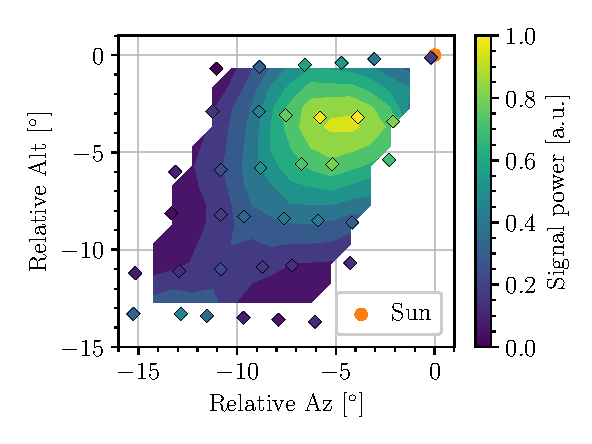
\includegraphics[scale=1]{figures/calibration_contour.pdf}
    \caption{Interpolation of signal power measured in the proximity of the Sun.}
    \label{fig:calibration_contour}
\end{figure}

\subsection{Distinguishing signal and noise}
The signal received by the antenna inherently contains noise which must be removed for the data to be properly analysed.
To this end, a signal measure was taken with the telescope pointed towards a nearby building, so that the registered spectrum  contained only the noise characteristic of the telescope location, which is expected to be found in all the signals received by the antenna.
The spectra of all the subsequently acquired signals were then divided by this noise spectrum, obtaining  signal-to-noise ratios which were further cleaned up by applying a moving average filter of $5$ bins of width.
An example of the application of this pipeline is depicted in \autoref{fig:process_example}.
\begin{figure}
    \begin{subfigure}{0.49\textwidth}
        \centering
        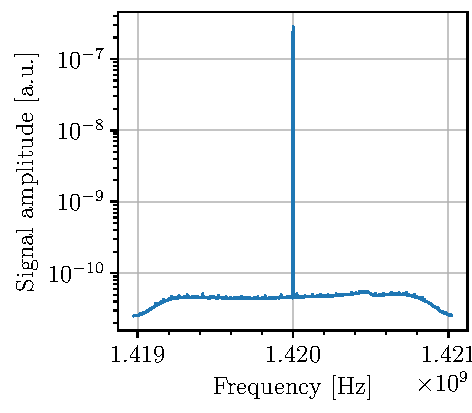
\includegraphics[scale=1]{figures/raw_signal.pdf}
        \caption{}
        \label{fig:raw_signal}
    \end{subfigure}
    \begin{subfigure}{0.49\textwidth}
        \centering
        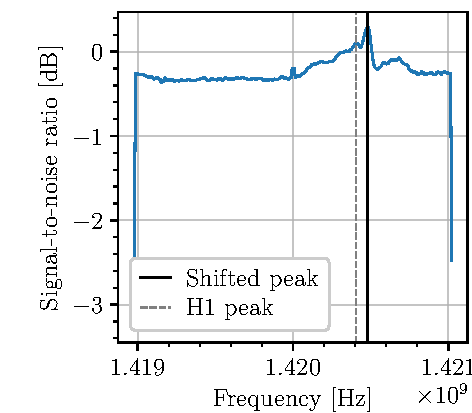
\includegraphics[scale=1]{figures/clean_signal.pdf}
        \caption{}
        \label{fig:clean_signal}
    \end{subfigure}
    \caption{(a) Measured signal pointing in $\ell = (30 \pm 1)^{\circ}$ and $b = (0 \pm 1)^{\circ}$ and (b) signal after processing.}
    \label{fig:process_example}
\end{figure}


\subsection{Velocity curve of the Milky Way}
A scan of the Milky Way was acquired by pointing VEGA to Galactic coordinates $b = (0\pm 1)^\circ$ and $18^\circ \leq \ell \leq 135^\circ$, spanning almost half of the galactic plane. The region $180^\circ < \ell < 360^\circ$ was never visible at the time of the measurements.
Using multiple gaussian fits \hl{TODO: Mettre plots des fits VEGA/SALSA dans l'annexe}, the frequency shift of the HI line and thus the radial relative velocity $V_r$ of the object for each spectrum was found. The methods presented in \autoref{sec:velocity_of_clouds} were used to derive the velocity of the hydrogen cloud observed, its distance from the Galactic Center and its distance from the Solar System.
\autoref{fig:VEGA_velocity_curve} depicts the velocity curves obtained for each method. For $R < R_0$, the velocity seems to grow linearly up to around $V=180$ km/s. In the region $R > R_0$, multiple behaviors are observed: one branch remains approximately constant at around $240$ km/s, while another branch grows linearly to above \mbox{$500$ km/s.}

By combining the distance of the hydrogen from Earth and the angle at which the measurements were taken, a map of the observed regions of the Galaxy was produced as shown in \autoref{fig:VEGA_galaxy_map}. One can see how a spiral pattern was produced by the data. \hl{compare with NASA map?}


\begin{figure}[htbp]
    \begin{minipage}[t]{0.5\textwidth}
        \centering
        \captionsetup{width=.95\textwidth}
        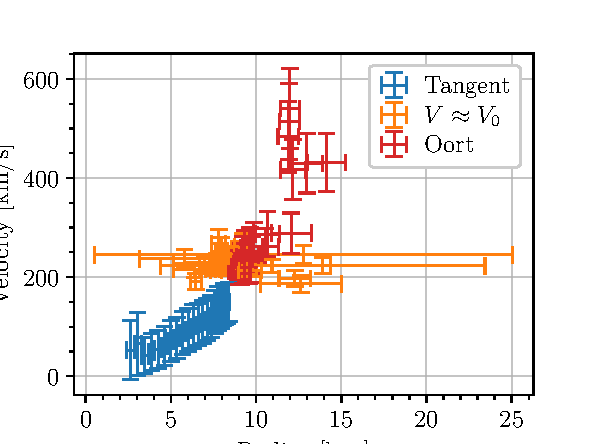
\includegraphics[scale=1]{figures/VEGA2_velocity_curve.pdf}
        \caption{Velocity curve of the Milky Way as measured by VEGA, using three different methods.}
        \label{fig:VEGA_velocity_curve}
    \end{minipage}
    \begin{minipage}[t]{0.5\textwidth}
        \centering
        \captionsetup{width=.95\textwidth}
        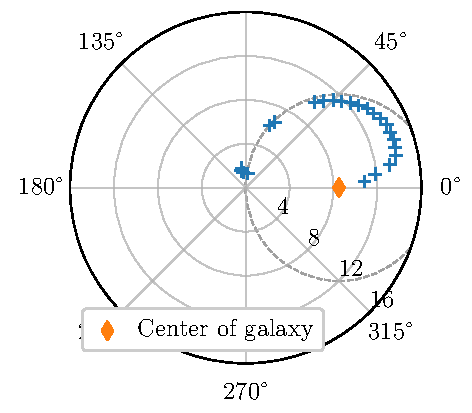
\includegraphics[scale=1]{figures/VEGA_galaxy_map.pdf}
        \caption{Position of the hydrogen clouds observed by VEGA, as derived from \autoref{eq:general_radius}. \hl{le cercle en traitillé peut être moins dense et il faut meilleur position de labels}}
        \label{fig:VEGA_galaxy_map}
    \end{minipage}
\end{figure}

\subsection{Comparing with SALSA}
Since VEGA  has never undergone extensive testing, the data analysis pipeline was tested with the remote operation of a more mature telescope: \emph{Torre}, one of the three SALSA (Such A Lovely Small Antenna) radio telescopes, based in the Onsala Observatory, Sweden.
It is an antenna of similar size and conception as VEGA, making it a nice comparison point. Using the same steps as outlined above, the velocity curve and a map of the observed region of the Galaxy was produced, shown in \autoref{fig:SALSA_velocity_curve} and \autoref{fig:SALSA_galaxy_map}.

\begin{figure}[htbp]
    \begin{minipage}[t]{0.5\textwidth}
        \centering
        \captionsetup{width=.95\textwidth}
        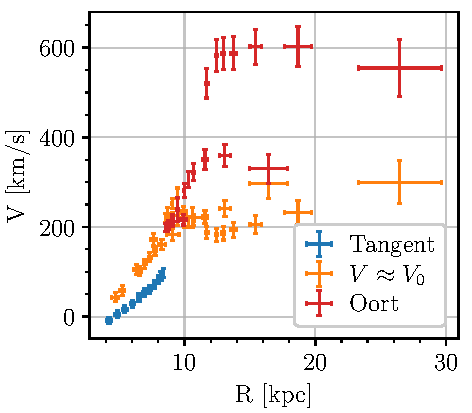
\includegraphics[scale=1]{figures/SALSA_velocity_curve.pdf}
        \caption{Velocity curve SALSA}
        \label{fig:SALSA_velocity_curve}
    \end{minipage}
    \begin{minipage}[t]{0.5\textwidth}
        \centering
        \captionsetup{width=.95\textwidth}
        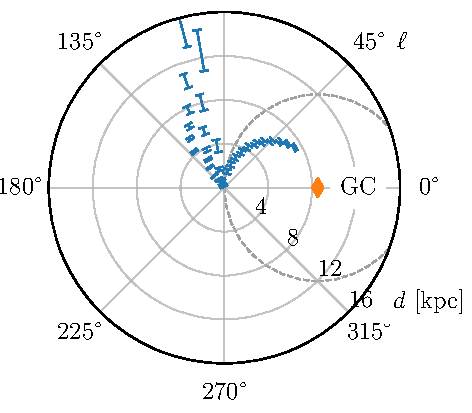
\includegraphics[scale=1]{figures/SALSA_galaxy_map.pdf}
        \caption{Galaxy map SALSA \hl{le cercle en traitillé peut être moins dense et il faut meilleur position de labels}}
        \label{fig:SALSA_galaxy_map}
    \end{minipage}
\end{figure}